\documentclass[../../main/main.tex]{subfiles}
\begin{document}

\section{Parameter Analysis}

\subsection{Effect of Increasing $U$}

\subsubsection{Expected Payoff of Value-Betting Hands}

It may seem unsurprising that strong hangs become less likely to get called as limits increase, but what about the actual expected payoff of these hands? Does the expected value of a specific hand strength in the unique admissible Nash equilibrium continue increasing as we increase $U$? The answer is no. In fact, for any fixed hand strength $x$, the expected payoff of that hand increases in $U$ only for up to a certain threshold, after which it decreases (see Figure \ref{fig:ev_x_vs_U}). This feels counterintuitive; increasing $U$ only gives the bettor more options, so how is it possible that the expected payoff of individual hands decreases? And which hands are gaining expected payoff to offset this? This is a surprising result, and it is worth exploring in more detail.

\begin{figure}[h!]
    \centering
    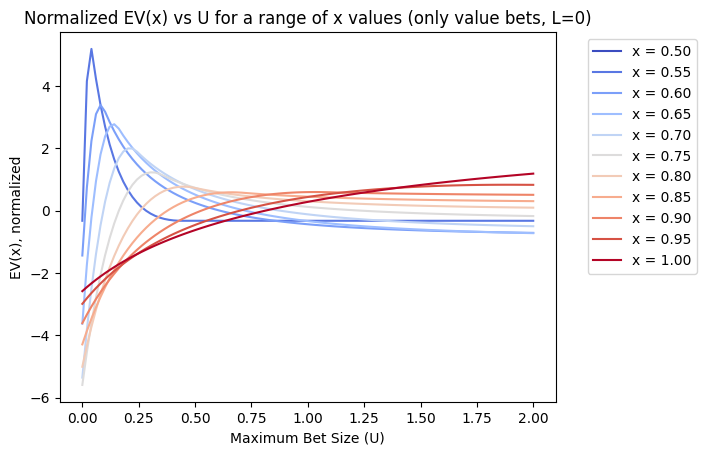
\includegraphics[width=\textwidth]{images/ev_vs_U.png}
    \caption{Expected value of a value-betting hand $x$ versus the upper limit $U$ in Nash equilibrium. Notice that each curve is increasing in $U$ up to some maximum, after which it decreases.Recall that $EV(x)$ denotes the expected payoff of a value-betting hand $x$ in the unique admissible Nash equilibrium.}
    \label{fig:ev_x_vs_U}
\end{figure}



\begin{theorem}
    \label{thm:payoff_increasing}
    For any value-betting hand strength $x$ and any $L, U$, $\frac{d}{dU} EV(x) < 0$ if 
    
    $$x < \max\left(v(U), \frac{1}{2(1+U)} \left( U \frac{\partial x_2}{\partial U} + \frac{U^2 + x_2(1 + 2U)}{1+U} \right) \right),$$

    and $\frac{d}{dU} EV(x) > 0$ otherwise.
\end{theorem}

To parse this in english: if we fix the bettor's hand strength $x$, the expected payoff to the bettor in the unique admissible Nash Equilibrium is decreasing in $U$ if $x$ falls below a certain threshold, but increasing in $U$ if $x$ is above this threshold. Specifically, this threshold is greater than the hand strength $v(U)$ which bets the maximum. 

Before proving the theorem, we will walk through some lemmas which explore how all the relevant variables change as we increase $U$, including the bluffing threshold $x_2$, the bet size $v^{-1}(x)$, and the calling cutoff $c(s)$.

\subsubsection{Bluffing Threshold}

We begin by showing that $x_2$, the boundary hand strength between bluffing and checking, is increasing in $U$. This means that for fixed $L$, increasing the upper limit $U$ makes the bettor bluff with more hands. 

\begin{lemma}
    \label{lem:x2_increasing}
    For any $L, U$,
    $$ \frac{d x_2}{d U} > 0. $$
\end{lemma}

\begin{customproof}
    Recall that $x_2$ is given by:

    \[ x_2 = \frac{r^{3} + t^{3} - 1}{r^{3} + t^{3} - 7} \]

    where $r = L/(1+L)$ and $t = 1/(1+U)$. We can use the chain rule to differentiate $x_2$ with respect to $U$:

    \[ \frac{d x_2}{d U} = \frac{\partial x_2}{\partial t} \frac{d t}{d U}. \]

    Note that $r$ has no dependence on $U$. We compute:

    \[ \frac{\partial x_2}{\partial t} = \frac{-18 t^{2}}{\left(r^{3} + t^{3} - 7\right)^{2}}, \quad \frac{d t}{d U} = - \frac{1}{(1+U)^2}. \]

    Therefore,

    \[ \frac{d x_2}{d U} = \frac{-18 t^{2}}{\left(r^{3} + t^{3} - 7\right)^{2}} \cdot \left(- \frac{1}{(1+U)^2}\right) = \frac{18 t^{2}}{(1+U)^2\left(r^{3} + t^{3} - 7\right)^{2}} > 0, \]

    which is positive since $r, t \in (0, 1)$ implies $r^3 + t^3 - 7 < 0$.

\end{customproof}

\subsubsection{Bet Size}

We now show that if we fix $x$ at any intermediate value-betting hand strength (betting neither the minimum nor maximum bet size) and then increase $U$, the bet size $s$ made by $x$ decreases. The intermediate value-betting hands are exactly $x \in [x_3, v(U)]$ and their bet sizes are given by $s = v^{-1}(x)$, so we get the following lemma:

\begin{lemma}
    \label{lem:v_inverse_decreasing}
    For any fixed $x \in [x_3, v(U)]$, 
    \[ 
        \frac{d}{dU} v^{-1}(x) < 0
    \]
\end{lemma}

\begin{customproof}
    Recall that
    $$v^{-1}(x) = -\frac{\sqrt{(4 x-4) (2 x_2-2)}}{4 x-4}-1,$$
    where $x_2 = \frac{r^3 + t^3 - 1}{r^3 + t^3 - 7}$ with $t = 1/(1+U)$. Importantly, $v^{-1}(x)$ is only dependent on $U$ through $x_2$, which in turn depends on $U$ only through $t$. Using the chain rule:
    \begin{align*}
        \frac{d}{dU} v^{-1}(x) & = \frac{\partial v^{-1}(x)}{\partial x_2} \frac{\partial x_2}{\partial t} \frac{dt}{dU}
    \end{align*}

    We compute each factor:

\begin{align*}
    \frac{\partial v^{-1}(x)}{\partial x_2} & = - \frac{1}{\sqrt{(4 x-4) (2 x_2-2)}} = - \frac{1}{(v^{-1}(x)+1)(4-4x)} < 0
\end{align*}

    which is negative since $x \in [0, 1]$ and $v^{-1}(x) >0$. From Lemma \ref{lem:x2_increasing}, we know that $\frac{\partial x_2}{\partial t} \frac{dt}{dU} > 0$.

    Therefore, the product of the three terms is always negative, so the bet size of intermediate bets is decreasing in $U$.
\end{customproof}

\subsubsection{Calling Cutoff}

Recall that $c(s)$ is defined as the minimum hand strength $y$ which should call a bet of size $s$ and is given in Nash equilibrium by:

$$c(s) = \frac{x_2 + s}{s+1}$$

We are specifically interested in how $c(v^{-1}(x))$ varies with $U$ for $x \in [x_3, v(U)]$, since this represents how the calling cutoff changes both directly from a strategic change, as well as indirectly due to the lower bet size $s$. It turns out that the calling cutoff is increasing in $U$ for all $x \in [x_3, v(U)]$. This is surprising because we just showed that the bet size $s$ is decreasing in $U$, and we expect smaller bets to be called more often. For reasons we will see later, this effect is overpowered by a strategic shift for the caller, who calls less often for all bet sizes as $U$ increases. 

\begin{lemma}
    \label{lem:c_increasing}
    For any fixed $x \in [x_3, v(U)]$, 
    \[ 
        \frac{d}{dU} c(v^{-1}(x)) > 0
    \]
\end{lemma}

\begin{customproof}
    As mentioned above, $c(s) = \frac{x_2 + s}{s+1}$ is dependent on $U$ in two distinct ways: directly through $x_2 = x_2(t)$ where $t = 1/(1+U)$, and indirectly through the bet size $s = v^{-1}(x)$. We use the multivariate chain rule:
    \begin{align*}
        \frac{d}{dU} c(v^{-1}(x)) & = \frac{\partial c(s)}{\partial s} \frac{d v^{-1}(x)}{d U} + \frac{\partial c(s)}{\partial x_2} \frac{\partial x_2}{\partial t} \frac{dt}{dU}
    \end{align*}

    The partial derivatives of $c(s)$ are:

    $$ \frac{\partial c(s)}{\partial s} = \frac{1-x_2}{(s+1)^2} \; \; \; \text{and} \; \; \; \frac{\partial c(s)}{\partial x_2} = \frac{1}{s+1}. $$

    Substituting $s = v^{-1}(x)$, we can simplify the first term using the fact that $(v^{-1}(x)+1)^2 = (1-x_2)/(2-2x)$:

    \begin{align*}
        \frac{\partial c(s)}{\partial s} \bigg|_{s=v^{-1}(x)} & = \frac{1-x_2}{(v^{-1}(x)+1)^2} = 2-2x
    \end{align*}

    From Lemma \ref{lem:v_inverse_decreasing}, we have:

    $$ \frac{d v^{-1}(x)}{d U} = \frac{\partial v^{-1}(x)}{\partial x_2} \frac{\partial x_2}{\partial t} \frac{dt}{dU} = \frac{-1}{(v^{-1}(x)+1)(4-4x)} \frac{\partial x_2}{\partial t} \frac{dt}{dU}. $$

    Substituting everything:

    \begin{align*}
        \frac{d}{dU} c(v^{-1}(x)) & =
        (2-2x) \cdot \frac{-1}{(v^{-1}(x)+1)(4-4x)} \cdot \frac{\partial x_2}{\partial t} \frac{dt}{dU}
        + \frac{1}{v^{-1}(x)+1} \cdot \frac{\partial x_2}{\partial t} \frac{dt}{dU}\\
        & = \frac{1}{v^{-1}(x)+1} \cdot \frac{\partial x_2}{\partial t} \frac{dt}{dU} \cdot \left( -\frac{2-2x}{4-4x} + 1\right) \\
        & = \frac{1}{v^{-1}(x)+1} \cdot \frac{\partial x_2}{\partial t} \frac{dt}{dU} \cdot \frac{1}{2}
    \end{align*}

    All three factors are positive: $v^{-1}(x) > 0$, and by Lemma \ref{lem:x2_increasing}, $\frac{\partial x_2}{\partial t} \frac{dt}{dU} > 0$. Therefore, the calling cutoff is increasing in $U$ for all $x \in [x_3, v(U)]$.

\end{customproof}

\subsubsection{Proof of Theorem \ref{thm:payoff_increasing}}

Having these tools, we can now finally return to the proof of Theorem \ref{thm:payoff_increasing}.

\begin{customproof}
    Recall the expected payoff of a value-betting hand $x$:

    \begin{align*}
        EV(x) & = \frac{1}{2} c(s) + (x - c(s)) \left(s+\frac{1}{2}\right) + (1-x) \left(-s-\frac{1}{2}\right)
    \end{align*}

    We break the proof into two cases:

    \textbf{Case 1 ($x > v(U)$):} In this case, hand $x$ bets the maximum amount $U$. Recall that $c(s)$ is implicitly a function of $s$ and $x_2$, which is itself a function of $U$. Using the multivariate chain rule, the derivative at $s=U$ is:

    \begin{align*}
        \frac{d}{dU} EV(x) & = \frac{\partial EV(x)}{\partial s} \bigg|_{s=U} + \frac{\partial EV(x)}{\partial c(s)} \left( \frac{\partial c(s)}{\partial s} + \frac{\partial c(s)}{\partial x_2} \frac{\partial x_2}{\partial U} \right) \bigg|_{s=U} \\
        & = \left( \frac{\partial EV(x)}{\partial s} + \frac{\partial EV(x)}{\partial c(s)} \frac{\partial c(s)}{\partial s}\right)\bigg|_{s=U}   +  \left( \frac{\partial EV(x)}{\partial c(s)} \frac{\partial c(s)}{\partial x_2} \frac{\partial x_2}{\partial U} \right) \bigg|_{s=U}
    \end{align*} 

    We want to know exactly when the above expression is positive. The partial derivatives to plug in are:

    \begin{align*}
        \frac{\partial EV(x)}{\partial s} & = 2x - 1 - c(s) \\
        \frac{\partial EV(x)}{\partial c(s)} & = - s \\ 
        \frac{\partial c(s)}{\partial s} & = \frac{1-x_2}{(s+1)^2} \\
        \frac{\partial c(s)}{\partial x_2} & = \frac{1}{s+1} \\
    \end{align*}

    We can leave $\frac{\partial x_2}{\partial U}$ as a free variable for now, since it is always positive by Lemma \ref{lem:x2_increasing}, and is independent of $x$. Plugging these in and rearranging terms, we can say that $EV(x)$ is increasing in $U$ if 

    \begin{align*}
        x & > \frac{1}{2(1+U)} \left( U \frac{\partial x_2}{\partial U} + \frac{U^2 + x_2(1 + 2U)}{1+U} \right)
    \end{align*}

    Where nothing on the right hand side is dependent on $x$. This means that for any fixed $L, U$, this gives a threshold value for $x$ below which $EV(x)$ is decreasing in $U$, and above which it is increasing in $U$.

    \textbf{Case 2 ($x_3 < x < v(U)$):} In this case, hand $x$ makes an intermediate-sized bet $s = v^{-1}(x)$. There are two distinct factors influencing the derivative $\frac{d}{dU} EV(x)$, namely the change in bet size $s = v^{-1}(x)$ and the change in calling cutoff $c(v^{-1}(x))$. By the multivariate chain rule, we can express the derivative as:

    \begin{align*}
        \frac{d}{dU} EV(x) & = \frac{\partial EV(x)}{\partial s} \frac{d v^{-1}(x)}{d U} + \frac{\partial EV(x)}{\partial c(s)} \frac{d c(v^{-1}(x))}{\partial U}
    \end{align*}

    The partial derivatives of $EV(x)$ are:

    \begin{align*}
        \frac{\partial EV(x)}{\partial s} & = 2x - 1 - c(s) \\
        \frac{\partial EV(x)}{\partial c(s)} & = - s
    \end{align*}

    The second is clearly negative. We can verify that the first must be positive if we go back to the constraints which gave us the Nash equilibrium. For the bet size $v^{-1}(x)$ to be optimal, we required that 

    $$ -s \frac{\partial c(s)}{\partial s} - c(s) + 2v(s) - 1 = 0,$$

    or equivalently, if we substitute $s= v^{-1}(x)$ and $v(s) = x$ and rearrange:

    $$ 2x -1 -c(v^{-1}(x)) = v^{-1}(x) \frac{\partial c(s)}{\partial s} > 0,$$

    since $\frac{\partial c(s)}{\partial s} = \frac{1-x_2}{(s+1)^2} > 0$, and $s$ is positive by definition.

    We know from Lemma \ref{lem:v_inverse_decreasing} that $\frac{d v^{-1}(x)}{d U} < 0$ and from Lemma \ref{lem:c_increasing} that $\frac{d c(v^{-1}(x))}{\partial U} > 0$.

    Combining everything, we see that both terms in $\frac{d}{dU} EV(x)$ are products of negative and positive, making both terms negative. Therefore, the expected payoff is decreasing in $U$ for all $x \in [x_3, v(U)]$.

\end{customproof}


\end{document}